\chapter{Einleitung}

\section{Motivation und Problemstellung}

Die digitale Transformation verändert sowohl das private als auch das geschäftliche Umfeld grundlegend. Das stellt auch die eher träge auf Veränderungen reagierende deutsche Versicherungsbranche vor neue Herausforderungen. So erleichtert die Digitalisierung Kunden den Zugang zu Informationen, beschleunigt Abschlussprozesse und ermöglicht das Vergleichen von Anbietern. Besonders deutlich zeichnen sich diese Veränderungen in der Kfz-Versicherungsbranche ab. So hat eine Studie von Statista aus dem Jahr 2022, in der 6027 Personen im Alter von 18-64 Jahren befragt wurden, ergeben, dass die Kfz-Versicherungssparte mit mehr als 25 \% online abgeschlossener Verträge in Deutschlandland in Versicherungsbranche aktuell führend ist.

Bei der Wahl des Anbieters ist dabei für die Kunden der Preis der ausschlaggebende Faktor, weshalb Kfz-Versicherer ihre Kosten reduzieren müssen, um für neue Kunden attraktiv zu bleiben. Diese Vergleichbarkeit bei sehr ähnlichen Produkten führt ebenfalls dazu, dass in Deutschland 2022 29 \% der Versicherungsnehmer ihren Kfz-Versicherungsanbieter wechselten. Eine Ursache hierfür ist der mangelnde Kundenkontakt und die daraus resultierende niedrige Kundenloyalität. Kfz-Versicherer haben hier das Problem, dass sie mit dem Kunden in der Regel nur beim Vertragsabschluss und im Schadenfall Kontakt haben. Daher ist es laut dem Vertriebsvorstand der Neodigital Versicherung AG Stephen Voss umso wichtiger, dass die wenigen Kontaktpunkte einfach, schnell und praktisch ablaufen, sodass der Versicherungsanbieter von Kunden nicht negativ wahrgenommen wird. 

Folglich müssen Kfz-Versicherer ihre internen Prozesse zur Kostenreduktion optimieren und ihren digitalen Auftritt verbessern, um  langfristig am Markt wettbewerbsfähig zu sein. Für diese digitale Transformation ist nicht eine einzelne Komponente entscheidend, sondern benötigen die Kfz-Versicherer vielmehr eine digitale Plattform, mit der interne Prozesse digitalisiert, Anwendungen integriert und zudem das Anbieten von weiteren Services für den Endkunden ermöglicht wird.

%\newpage
\section{Zielsetzung und Abgrenzung}

Die SAP Business Technology Plattform ist eine solche digitale Plattform mit der Unternehmen ihre bestehende IT-Landschaft transformieren und an neue Geschäftsanforderungen anpassen können. 

Ziel dieser Arbeit ist es daher die Anforderungen der Kfz-Versicherer an eine digitale Plattform zu identifizieren, um anschließend beurteilen zu können, inwiefern die Anforderungen der Kfz-Versicherer an eine digitale Plattform von der SAP Business Technology Plattform erfüllt werden. Die aus der Analyse resultierende Handlungsempfehlung soll Kfz-Versicherern eine praxisorientierte Vorgehensweise zur Implementierung der SAP Business Technology Plattform aufzeigen.

Dabei wird der deutsche Kfz-Versicherungsmarkt betrachtet, da eine Analyse inklusiver internationaler Märkte aufgrund der unterschiedlichen regulatorischen Anforderungen sowie der unterschiedlichen Preisgestaltung/ Digitalisierungsgrad / Tarifierung(smerkmale) \improvement{Frage an Bernd: Welchen Punkt würdest du hier noch aufführen?} nicht aussagekräftig wäre. Des Weiteren konzentriert sich die Arbeit im Wesentlichen auf die technologischen Merkmale einer digitalen Plattform. Darüber hinaus wird im Rahmen dieser Untersuchung digitaler Plattformen als Wettbewerbsfaktor betrachtet, nicht aber in Bezug zu anderen Wettbewerbskräften im Versicherungsmarkt gesetzt.

\newpage
\section{Aufbau der Arbeit}

\begin{figure}[h]
    \centering
    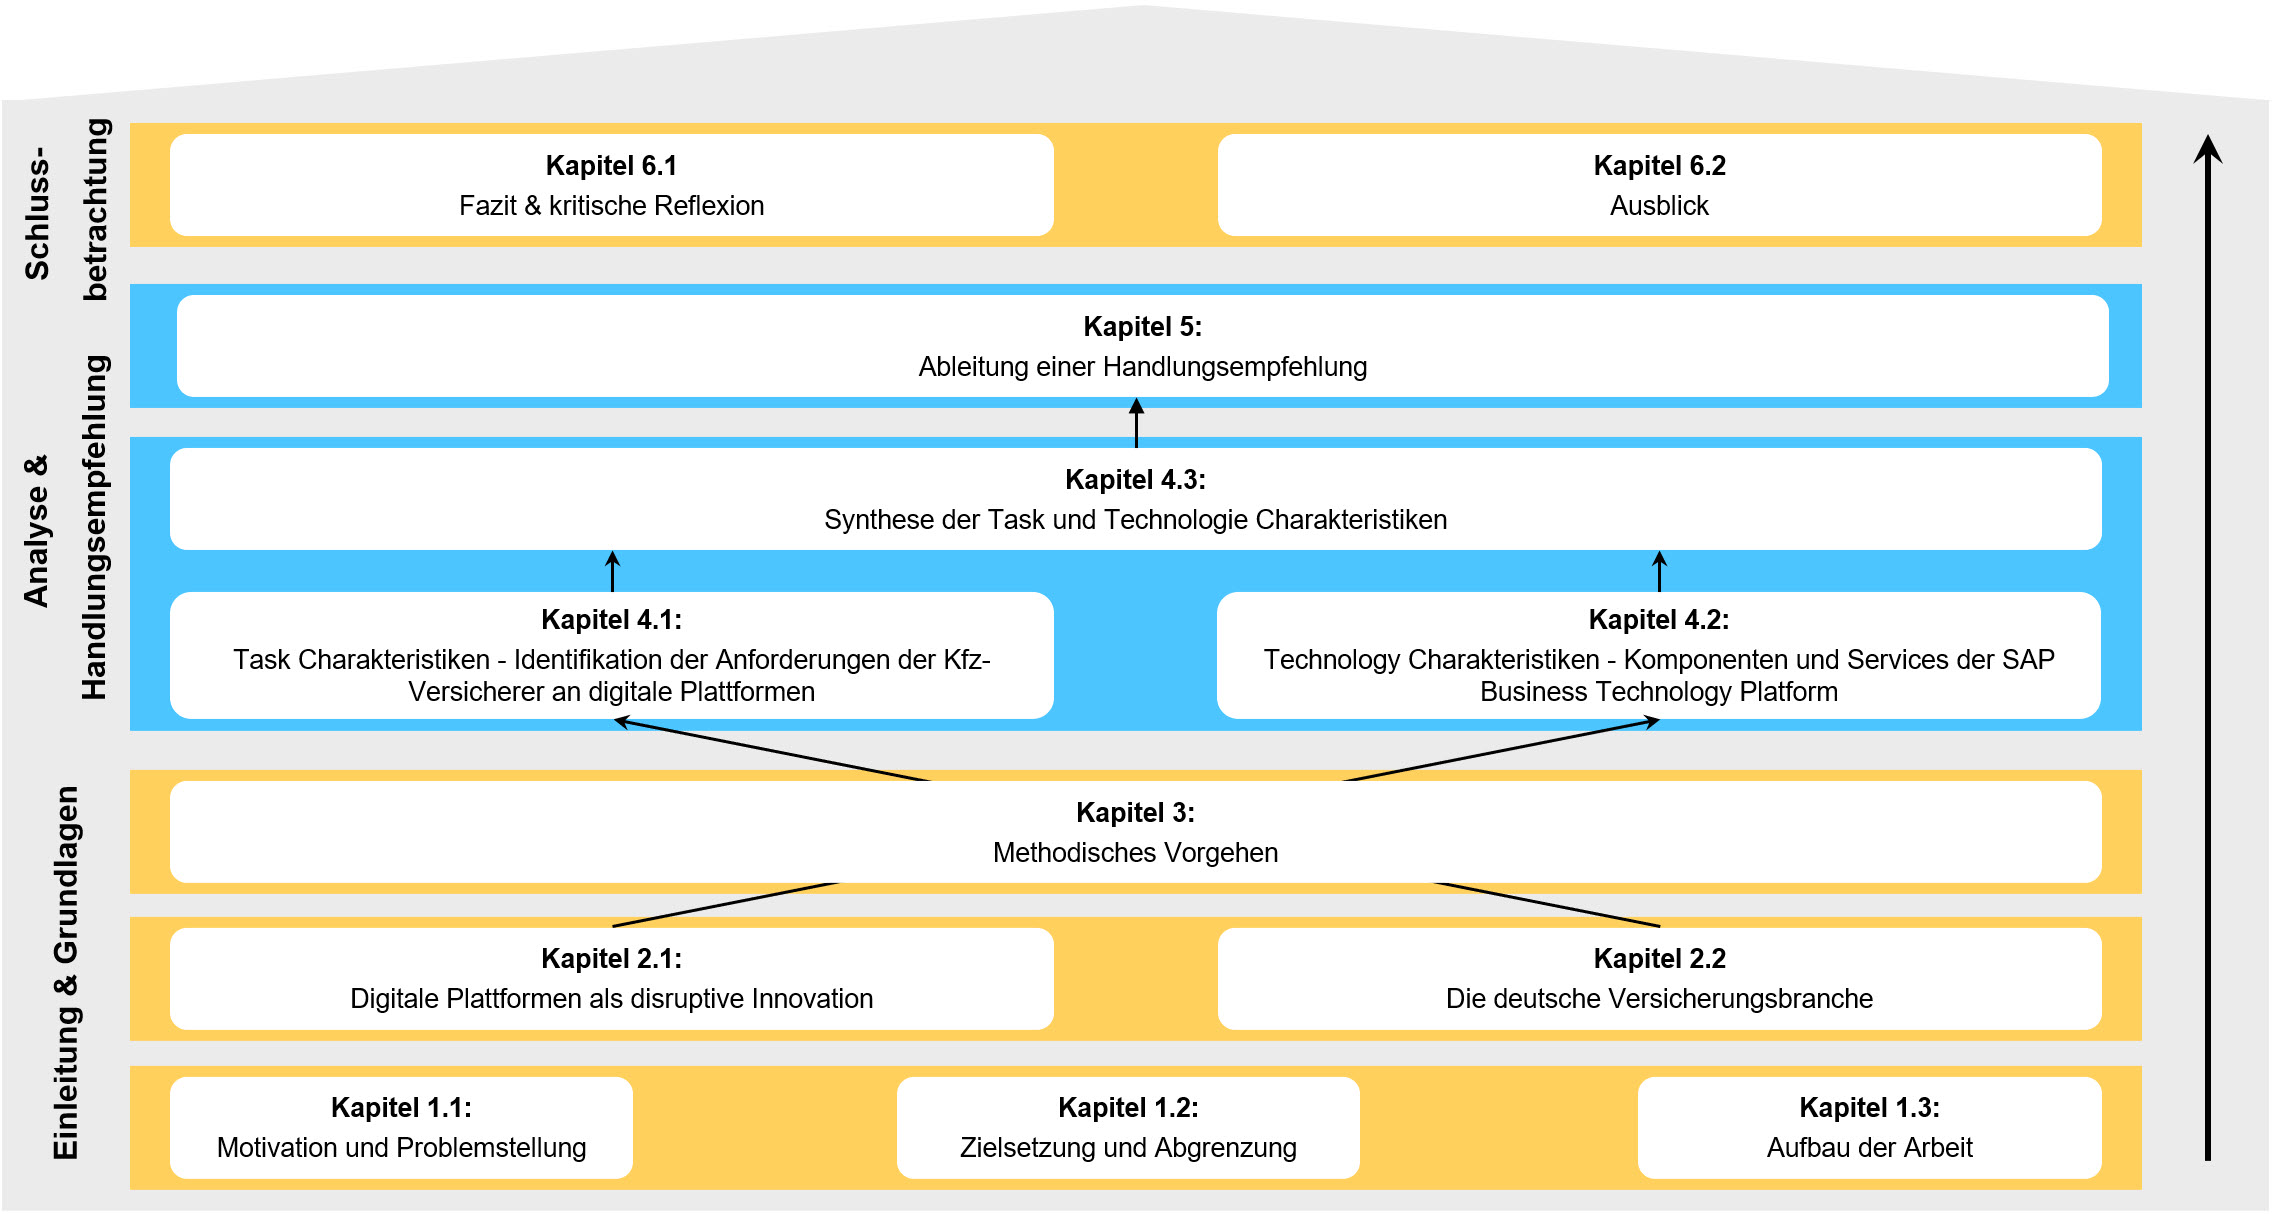
\includegraphics[width=1\textwidth]{img/Aufbau_der_Arbeit.jpg}
    \caption[Aufbau der Arbeit]{Aufbau der Arbeit\autocite{Aufbau}}
    \label{fig:Aufbau}
\end{figure}
\footnotetext{eigene Darstellung}

\improvement{Feedback Bernd: Pfeile nicht überkreuzen und Bild größer}

...Text kommt noch...

\newpage